%/**
% * @file tese.tex
% * @brief This file have the configuration parameters of Dr. Degree thesis.
% * @ingroup Documentation
% * @author $Author: rodcosta $
% * @date $Date: 2009/07/12 18:54:10 $
%**
\documentclass[12pt,a4paper,oneside,final]{book}
%%% para vers\~{o}es parciais do dumento final utilizar:
%\documentclass[12pt,a4paper,draft]{book}
%\documentclass[12pt,a4paper,twoside,fleqn,draft]{book}
%%%%%%%%%%%%%%%%%%%%%%%%%%%%%%%%%%%%%%%%%%%%%%%%%%%%%%%%%%%%%%%%
%%% PREAMBULO DO DOCUMENTO COME\c{C}A AQUI
%\usepackage{natbib}
%\bibliographystyle{elsart-harv}
%inclui coisas da abnt
%\bibliographystyle{abntcite}
%\usepackage{hvfoat}
\usepackage{datetimepor}
\usepackage{monografia}
\usepackage{multicol}
\usepackage{rotating}
\usepackage{monografia_defs}
\usepackage[none]{hyphenat}
\usepackage[latin1]{inputenc}
\usepackage{assinatura}
\usepackage{color}
\usepackage{multirow}
% \bibstyle{abnt-alf}
\usepackage{sidecap}
\usepackage{ifthen}
\usepackage{psfrag}
\usepackage{supertabular}
\usepackage[subfigure]{tocloft}

% Permite utilizar configuracoes da linguagem portugesa do Brasil e Inglesa
\usepackage[english,brazil]{babel}
% Permite especificar codificacao das entradas (caracteres acentuados - � - sem usar \'a)
%\usepackage[latin1]{inputenc}
% Permite utiliza��o de referencias cruzadas
\usepackage[brazil]{varioref}
\usepackage[T1]{fontenc}
%
\usepackage{listings}             % Include the listings-package




\newcommand{\titulo}{Estudo comparativo das plataformas Android e iOS para aplica��es RESTful}
\newcommand{\autor}{Tiago Augusto da Silva Bencardino}
\newcommand{\orientador}{Prof. Dr. Jos� Marques Soares}
\newcommand{\coorientador}{Prof. }
\newcommand{\membroa}{Prof. p1}
\newcommand{\membrob}{Prof. p2}
\newcommand{\membroc}{Prof. p3}
\renewcommand{\eqref}[1]{equa\c{c}\~{a}o~\ref{#1}}
\newcommand{\eqrefp}[1]{equa\c{c}\~{o}es~\ref{#1}}
\newcommand{\ok}{$\blacksquare$}
\newcommand{\nok}{$\square$}

\newcommand{\secao}{\section}
\newcommand{\capitulo}{\chapter}
\newcommand{\subsecao}{\subsection}

\newcommand{\secref}[1]{se\c{c}\~{a}o~\ref{#1}}
\newcommand{\secrefp}[1]{se\c{c}\~{o}es~\ref{#1}}
\newcommand{\tabref}[1]{Tabela~\ref{#1}}
\newcommand{\tabrefp}[1]{Tabelas~\ref{#1}}
\newcommand{\figref}[1]{Figura~\ref{#1}}
\newcommand{\figrefp}[1]{Figuras~\ref{#1}}
\newcommand{\quadro}[1]{Quadro~\ref{#1}}
\usepackage[breaklinks,final,pdftitle={\titulo},pdfauthor = {\autor}]{hyperref}

%\usepackage{hyperref}
\usepackage[sort]{cite}
\usepackage[alf,abnt-and-type=e,abnt-full-initials=no,abnt-last-names=abnt,abnt-etal-list=2,abnt-etal-text = emph]{abntcite}
\newcommand{\citet}[1]{\citeonline{#1}}

%\newcommand{\eqref}[1]{(\ref{#1})}
\newcolumntype{Y}{>{\centering\arraybackslash}X}
%\newcommand{\secref}[1]{se\c{c}\~{a}o~\ref{#1}}
%\newcommand{\secrefp}[1]{se\c{c}\~{o}es~\ref{#1}}
%\newcommand{\tabref}[1]{Tabela~\ref{#1}}
%\newcommand{\tabrefp}[1]{Tabelas~\ref{#1}}
%\newcommand{\figref}[1]{Figura~\ref{#1}}
%\newcommand{\figrefp}[1]{Figuras~\ref{#1}}
%
%\usepackage[dvips]{graphicx}
%\usepackage[portuges]{babel}
\usepackage[printonlyused]{acronym}
\usepackage{hvfloat}

\usepackage{tabularx}
\usepackage{here}
\usepackage{listings}
% Definindo novos tipos de lista
\usepackage{tocloft}
\usepackage{etoolbox}
%\newcommand{\listexamplename}{\textbf{\Huge{Lista de Quadros}}}
%\newlistof{example}{exp}{\listexamplename}
%\newcommand{\example}[1]{%
%    \refstepcounter{example}
%    \par\noident\textbf{Quadro \theexample.#1}
%    \addcontentsline{exp}{example}
%    {\protect\numberline{\theexample}#1}\par
%}
%
    \usepackage{longtable}
\usepackage{supertabular}

\hyphenation{defei-tuoso Fe-de-ral Uni-ver-si-da-de Dis-cos atri-bu-tos re-sul-ta-dos ar-ma-ze-na-men-to}
\hyphenation{tem-pe-ra-tu-ra sis-te-ma lei-tu-ra }


\begin{document}
%padronizacao
\DeclareGraphicsExtensions{.jpg,.pdf,.mps,.png}

%\usepackage[final]{pdfpages}
%\usepackage{Fancyhdr}
%\bibliographystyle{IEEEtranPor}
% \includeonly{capa,agradecimentos}
% \includeonly{capa_externa,capa}
%%% PREAMBULO DO DOCUMENTO ACABA AQUI
%%%%%%%%%%%%%%%%%%%%%%%%%%%%%%%%%%%%%%%%%%%%%%%%%%%%%%%%%%%%%%%%

%%%%%%%%%%%%%%%%%%%%%%%%%%%%%%%%%%%%%%%%%%%%%%%%%%%%%%%%%%%%%%%%
%%% CAPA

\pagenumbering{Roman}
\thispagestyle{empty}%

\begin{center}
    \includegraphics[width=2.5cm]{figs/ufc.jpg} \\%
    \textsc{
    Universidade Federal do Cear� \\%
    Departamento de Engenharia de Teleinform�tica \\%
    Curso de Gradua��o em Engenharia de Teleinform�tica\\
    }
    \vspace{2.5 cm}%
    {       \textbf{\autor}
    }\\%

    \null\vfill%%
    \vspace{.2cm}%
    {\Large         \textbf{\titulo}\\}


    \null\vfill%%
    \vspace{1 cm}%
    {\normalsize    \textsc{Fortaleza -- Cear� \\%
                            Fevereiro~2013 }}
\end{center}

% ----------------------------------------------------------------------- %
% Onde serão inseridas informações que irão aparecer na capa e na
% folha de rosto
%
% Arquivo: capa.tex
% ----------------------------------------------------------------------- %
%\capa
%%capa feita manualmente
%%-------------------------
\begin{titlepage}
\begin{center}

\includegraphics[scale=0.33]{fig/logo_UFC.eps}\\
\vfill
{\MakeUppercase{\instituicao}}\par
{\MakeUppercase{\departamento}}\par
{\MakeUppercase{\curso}}\\
\vfill
\begin{center}
\Large\MakeUppercase{\titulo}\par
\end{center}
\vfill\vfill
\begin{center}
{\MakeUppercase{\autor}}
\end{center}
\vfill\vfill\vfill

\setlength{\parskip}{.3cm}
{\normalfont{\Local}} \par
{\normalfont{\Data}}
\end{center}
\end{titlepage}
%%-------------------------
%Folha de rosto feita manualmente
%----------------------------------------
\thispagestyle{empty}
\vspace{1.1cm}
  \begin{center}
    \MakeUppercase{\autor}
  \end{center}
\vfill\vfill\vfill
   \begin{center}
     \Large\MakeUppercase{\titulo}\par
   \end{center}
   \vspace{.8cm}
   \hspace{.45\textwidth}
     \begin{minipage}{.5\textwidth}
         {\comentario}\par
     \end{minipage}
\vspace{.8cm}
\begin{center}
   Orientador: {\orientador}
   \vspace{0.7cm}
   \end{center}
\vfill
\begin{center}
  \setlength{\parskip}{.3cm}
     \setlength{\parskip}{0cm}
     {\MakeUppercase{\instituicao}}\par
	{\MakeUppercase{\departamento}}\par
	{\MakeUppercase{\curso}}\\
     \setlength{\parskip}{.3cm}\par
\end{center}
\vfill\vfill
\begin{center}
\setlength{\parskip}{.3cm}
{\normalfont{\Local}} \par
{\normalfont{\Data}}
\end{center}

%---------------------------------------
\thispagestyle{empty}%

\begin{center}
    %
\includegraphics[width=2.5cm]{figs/UFC.eps} \\%
    \textsc{ \autor } \\
     \vspace{.5 cm} \textbf{ \titulo }     \\
\end{center}
    \vspace{.2 cm}
    Esta Monografia foi julgada adequada para a obten\c{c}\~{a}o do diploma de Engenheiro do Curso de Gradua\c{c}\~{a}o em Engenharia de Teleinform\'{a}tica da Universidade Federal do Cear\'{a}.
    \assinatura{\autor}
    \vspace{2 cm}
     Banca Examinadora:
     \assinatura{\orientador ~(Orientador)\\ Universidade Federal do Cear\'{a} - UFC}
     \assinatura{Prof. Msc. Alexandre Moreira de Moraes  \\ Universidade Federal do Cear\'{a} - UFC}
     \assinatura{Prof. Dr. Danielo Gonçalves Gomes \\ Universidade Federal do Cear\'{a} - UFC}
%     \assinatura{\hspace{-0.5 cm} --}
%     \assinatura{\membroc}
%     \assinatura{\membrod}

     \vspace{5 cm}%\null\vfill%%


\begin{center}
    {\normalsize    Fortaleza, 22 de Fevereiro de 2013}
\end{center}

\frontmatter \pagestyle{roman}
%%%%%%%%%%%%%%%%%%%%%%%%%%%%%%%%%%%%%%%%%%%%%%%%%%%%%%%%%%%%%%%%
%%% RESUMO

% ----------------------------------------------------------------------- %
% Pequeno texto que em poucas palavras consegue expressar o trabalho.
% O resumo deve ser concebido de forma tal que, uma pessoa ao ler o resumo
% possa entender sobre qual assunto este trabalho trata.
%
% Arquivo: resumo.tex
% ----------------------------------------------------------------------- %
\pdfbookmark[1]{Resumo}{CHP:RESUM0}
\chapter*{Resumo}
\label{CHP:RESUM0}
\thispagestyle{empty}
\singlespacing
	\lipsum[3-4]
\onehalfspacing
% ----------------------------------------------------------------------- %
% Tradução do resumo para a língua inglesa.
% 
% 
%
% Arquivo: abstract.tex
% ----------------------------------------------------------------------- %
\pdfbookmark[1]{Abstract}{CHP:ABSTRACT}
\chapter*{Abstract}
\label{CHP:ABSTRACT}
\thispagestyle{empty}
\singlespacing
	\lipsum[5-6]
\onehalfspacing
%%%%%%%%%%%%%%%%%%%%%%%%%%%%%%%%%%%%%%%%%%%%%%%%%%%%%%%%%%%%%%%%
%%% DEDICATRIA
% ----------------------------------------------------------------------- %
% Pequena dedicatória ou uma epígrafe (uma citação pertinente ao seu 
% trabalho ou que represente o seu modo de pensar.) 
% 
%
% Arquivo: dedicatoria.tex
% ----------------------------------------------------------------------- %
\thispagestyle{empty}
\vspace*{\fill}

{ \raggedleft


\textit{Dedico este trabalho a ...}

~
}

%%%%%%%%%%%%%%%%%%%%%%%%%%%%%%%%%%%%%%%%%%%%%%%%%%%%%%%%%%%%%%%%
%%% AGRADECIMENTOS
%% ----------------------------------------------------------------------- %
% Um pequeno texto para agradecer àqueles que contribuíram de maneira
% relevante à elaboração do trabalho 
%
% Arquivo: agradecimentos.tex
% ----------------------------------------------------------------------- %

\chapter*{Agradecimentos}
\thispagestyle{empty}
\lipsum[1-2]

%\textbf{DEDICAT\'{O}RIA}
\thispagestyle{empty}%
\newpage
\null\vfill
\begin{flushright}
%\emph{"Fazer do of\'{\i}cio uma divers\~{a}o levada a s\'{e}rio."}\\Chico Science
\emph{$\ldots$ Cada sonho que voc� deixa pra tr�s, � um peda�o do seu futuro que deixa de existir.}\\
Steve Jobs

%\emph{ "$\ldots$\\All your life, You were only waiting for the moment to arise.\\
%%...
%%All your life, You were only waiting for the moment to be free.
%Black bird fly, black bird fly\\
%Into the light of the dark black night\\$\ldots$" }
%
%\emph{Black Bird - The Beatles}
\end{flushright}
   \vspace{3.0cm}

%% ----------------------------------------------------------------------- %
% Pequena dedicatória ou uma epígrafe (uma citação pertinente ao seu 
% trabalho ou que represente o seu modo de pensar.) 
% 
%
% Arquivo: dedicatoria.tex
% ----------------------------------------------------------------------- %
\thispagestyle{empty}
\vspace*{\fill}

{ \raggedleft


\textit{Dedico este trabalho a ...}

~
}

%%%%%%%%%%%%%%%%%%%%%%%%%%%%%%%%%%%%%%%%%%%%%%%%%%%%%%%%%%%%%%%%
%%% ABREVIA\c{C}\~{O}ES
\begin{singlespace}
    %%%%%%%%%%%%%%%%%%%%%%%%%%%%%%%%%%%%%%%%%%%%%%%%%%%%%%%%%%%%%%%%
    %%% \'{I}NDICE
    %\addtocontents{toc}{\noindent\protect\rule{\textwidth}{.2pt}\par}
    \pdfbookmark[1]{Sum�rio}{sumario_label} %\label{sumario_label}
    \tableofcontents%
    %%%%%%%%%%%%%%%%%%%%%%%%%%%%%%%%%%%%%%%%%%%%%%%%%%%%%%%%%%%%%%%%
    %%% LISTA DE FIGURAS
    \newpage
    %\pdfbookmark[1]{Lista de Figuras}
    \listoffigures%
    \addcontentsline{toc}{chapter}{Lista de Figuras}%
    %%%%%%%%%%%%%%%%%%%%%%%%%%%%%%%%%%%%%%%%%%%%%%%%%%%%%%%%%%%%%%%%
    %%% LISTA DE TABELAS
    \newpage
    \listoftables%
    \addcontentsline{toc}{chapter}{Lista de Tabelas}%
    %%%%%%%%%%%%%%%%%%%%%%%%%%%%%%%%%%%%%%%%%%%%%%%%%%%%%%%%%%%%%%%%
    %%% LISTA DE QUADROS
  %  \newpage
%    \addcontentsline{toc}{chapter}{Lista de Quadros}%
%    \chapter*{Lista de Quadros}%%
%    
Quadro 1

Quadro 2

Quadro 3

    %%%%%%%%%%%%%%%%%%%%%%%%%%%%%%%%%%%%%%%%%%%%%%%%%%%%%%%%%%%%%%%%
    %%% LISTA DE ALGORITMOS
    %    \listofalgorithms%
    %    \addcontentsline{toc}{chapter}{Lista de Algoritmos}%
     %\addtocontents{toc}{\noindent\protect\rule{\textwidth}{.2pt}\par}
    %%%%%%%%
    %%%% NOTA\c{C}\^{A}O
%    \addcontentsline{toc}{chapter}{Lista de S\'{\i}mbolos}%
%    \chapter*{Lista de S\'{\i}mbolos}%%
%    \LTXtable{\textwidth}{pretexto/simbolos}%%
    \newpage
    \addcontentsline{toc}{chapter}{Lista de Siglas}%
    \chapter*{Lista de Siglas}%%
    \include{pretexto/acronimos}
    %\LTXtable{\textwidth}{pretexto/siglas}%%
    %GATHER{pretexto/simbolos.tex}%%
    %GATHER{pretexto/siglas.tex}%%
\end{singlespace}

\pagestyle{capitulo} \setlength{\parskip}{1ex plus 0.5ex}
%%%%%%%%%%%%%%%%%%%%%%%%%%%%%%%%%%%%%%%%%%%%%%%%%%%%%%%%%%%%%%%%
%%% CAP�TULO 1: INTRODU��O
\mainmatter
\section{Introdução}\label{sec:intro}
\AtBeginSec

\begin{frame}{Elementos da Comunicação}
\begin{bigitem}
 \item A comunicação faz parte de nossa rotina diária:
 \begin{bigitem}
  \item chamada de telefone fixo ou móvel;
  \item e-mail na Internet;
  \item um programa de TV ou de rádio.
 \end{bigitem}
 \begin{figure}[!htb]
    \centering
    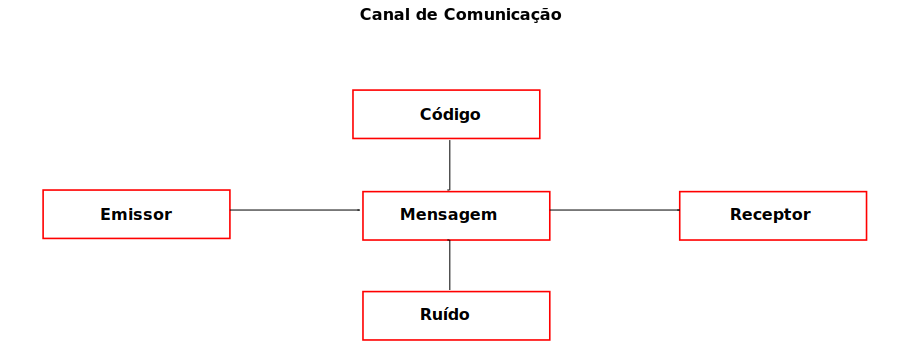
\includegraphics[width=0.50\linewidth]{../Imagens/elem_com.eps}
    \caption{Elementos do Processo de Comunicação.}\label{fig:elem_com}
   \end{figure}
\end{bigitem}
\end{frame}

\begin{frame}{Sistemas de Comunicações Atuais}
 \begin{bigitem}
  \item Como exemplo de sistemas de comunicações sem fio atuais, temos:
  \begin{bigitem}
    \item WLAN, Bluetooth, WiMAX
 \end{bigitem}
 \item Como exemplo de sistemas de comunicações móveis sem fio atuais, temos:
  \begin{bigitem}
   \item 2G, 3G, 4G.
 \end{bigitem}
 \end{bigitem}  
\end{frame}

\begin{frame}{Motivação}
 \begin{bigitem}
  \item O canal de comunicações móveis sem fio é cheio de desafios, desde a propagação até os serviços oferecidos.
  \item Para isso, é necessário um avanço nas técnicas utilizadas e nos dispositivos eletrônicos:
  \begin{bigitem}
    \item OFDM (Orthogonal Frequency-Division Multiplexing), MIMO (Multiple-Input and Multiple-Output).
    \item Microeletrônica.
  \end{bigitem}
  \item A potência de transmissão é um fator limitante em qualquer sistema de comunicações. 
 \end{bigitem}
\end{frame}

\begin{frame}{Motivação}
 \begin{bigitem}
  \item Para a nova geração, 4G, espera-se a utilização de técnicas de cooperação em conjunto com OFDM.
  \item É possível combinar técnicas de multiplexação e cooperação para um aumento da taxa de transmissão e um controle eficiente da potência de transmissão.
  \item Originam-se problemas atuais e relevantes do ponto de vista prático.
 \end{bigitem}
\end{frame}

\begin{frame}{Objetivos}
 \begin{bigitem}
  \item União de duas técnicas, multiplexação e cooperação:
  \begin{bigitem}
    \item utilização eficiente da potência de transmissão
    \item aumento da taxa.  
  \end{bigitem}
  \item É formulado um problema de otimização
  \begin{bigitem}
    \item  Objetivo:
    \begin{bigitem}
      \item  maximização da taxa
    \end{bigitem}
    \item Restrições:
    \begin{bigitem}
      \item potência em cada enlace (chamado na literatura de salto);
      \item emparelhamento dos canais (chamados de subportadoras).
    \end{bigitem}
  \end{bigitem}  
 \end{bigitem}
\end{frame}


%%%%%%%%%%%%%%%%%%%%%%%%%%%%%%%%%%%%%%%%%%%%%%%%%%%%%%%%%%%%%%%
%%%% CAP�TULO 2: Server-Side
\chapter{Fundamentacao}

\section{Servi�os PaaS}
\subsection{Defini��o }

Segundo o National Institute of Standarts and Technology (NIST), o termo computa��o em n�vem � referentea ``Cloud Computing � um modelo que permite de forma conveniente, o acesso � rede sob demanda para um conjunto compartilhado de recursos de computa��o configur�veis (por exemplo, redes, servidores, armazenamento, aplicativos e servi�os) que podem ser rapidamente provisionados e lan�ados  com o m�nimo de esfor�o de gest�o ou a intera��o de um prestador de servi�os.''. Um dos servi�os definidos � o PaaS, acr�nimo do ingl�s ``plataform as a service''.
	Ainda de acordo com o NIST, o PaaS � ``a capacidade fornecida ao consumidor de publicar aplica��es usando linguagem de programa��o, bibliotecas, servi�os suportados pelo provedor''. Com o fornecimento de tal servi�o, o consumidor n�o precisa se preocupar com o controle de certos servi�os de infra-estrutura, como a rede, servidores, sistemas operacionais, armazenamento, ou seja, criam uma camada de abstra��o de servi�os de infra-estrutura.
	
	De acordo com \url{http://broadcast.rackspace.com/hosting_knowledge/whitepapers/Understanding-the-Cloud-Computing-Stack.pdf}, servi�os PaaS possuem as seguintes caracter�sticas:
\begin{itemize}
\item Servi�os para desenvolver, testar, publicar, hospedar e manter aplica��es de forma integrada;
\item Arquitetura Multi-tenant, onde v�rios usu�rios podem utilizar o mesmo ambiente de desenvolvimento;
\item Constru��o garantindo escalabilidade, incluindo balanceamento de carga (load balancing) e replica��o de dados para recupera��o de falhas (failover);
\item Integra��o com webs services e banco de dados atrav�s de padr�es comuns;
\item Suporte para desenvolvimento em equipes, podendo ter ferramentas de planejamento de projetos e de comunica��o;
\item Ferramentas para gerenciamento dos custos.
\end{itemize}
Ou seja, sistemas PaaS s�o �teis para desenvolvedores individuais e startups, pois fornecem facilidade de publica��o sem os custos e complexidades de hardwares e softwares inerentes a uma aplica��o web comum. \url{http://www.guardian.co.uk/technology/2008/apr/17/google.software}.
	
\subsection{Heroku}

O Heroku uma plataforma cloud de servi�os PaaS, que roda sobre o Amazon EC2 (IaaS, infra-structure as a service), existente desde junho de 2007. Possui suporte para as seguintes linguagens: Ruby, Java, Node.JS, Scala, Clojure, Python e PHP. Internamente, roda sobre o sistema operacional Ubuntu.
Inicialmente, o Heroku foi desenvolvido com suporte exclusivo para a linguagem Ruby. Em julho de 2011, Matz Matsumoto, criador do Ruby, entrou para a empresa como Arquiteto-chefe e, nesse mesmo m�s, passou a dar suporte tamb�m para Node.js e Clojure.
Em setembro de 2011, a rede social Facebook fez uma parceria com o Heroku a fim de facilitar a publica��o de aplicativos para sua pr�pria plataforma \url{https://developers.facebook.com/blog/post/558}. Em poucos passos, � poss�vel criar uma aplica��o no Facebook e no Heroku, simultaneamente.
O Heroku usa uma unidade de m�quina virtual chamada ``Dyno'' com 4 cores e at� 512mb de RAM.

	

\section{REST}
REST, acr�nimo de Representional State Transfer, foi definido em uma tese de doutorado por Roy Fielding da seguinte maneira: 
``A REST (Transfer�ncia do Estado Representativo) � pretendida como uma imagem do design da aplica��o se comportar�: uma rede de websites (um estado virtual), onde o usu�rio progride com uma aplica��o selecionando as liga��es (transi��es do estado), tendo como resultado a p�gina seguinte (que representa o estado seguinte da aplica��o) que est� sendo transferida ao usu�rio e apresentada para seu uso.''

De modo geral, o REST � uma interface de comunica��o onde h� um provedor de servi�os e um consumidor. Tal interface pode ser descrita utilizando XML, HTTP, YAML, JSON ou at� mesmo texto puro, de modo a n�o utilizar trocas de mensagens complexas como o SOAP. 

O REST possui alguns princ�pios, a saber:
\begin{itemize}
\item Modelo provedor/consumidor Stateless (sem estado): cada mensagem HTTP trocada possui todas as informa��es necess�rias para a comunica��o, ou seja, nenhuma das partes necessita gravar estado da comunica��o. Em sistemas web, � comum o uso de cookies para manter o estado da sess�o; j� em sistemas mobile, � comum utilizarmos um token de autentica��o, com a mesma finalidade.

\item Opera��es HTTP: de modo a diminuir o tr�fego de dados, s�o utilizados m�todos HTTP para acessar os recursos de informa��o. As opera��es mais utilizadas s�o o GET, PUT, POST e DELETE. Em sistemas REST, � comum combinar tais m�todos com opera��es de CRUD (create, read, update e delete), que faz persist�ncia de dados em um determinado recurso ou entidade.

\item Identifica��o de recursos: As URIs identificam cada uma das entidades e seus elementos, ficando a cargo da opera��o HTTP definir a a��o a ser feita com cada um dos recursos ou elementos.

\item Uso de hiperm�dia: As trocas de mensagem de comunica��o � feita utilizando, no corpo da mensagem HTTP, uma linguagem de marca��o, conforme j� citado anteriormente. Por�m, n�o h� uma restri��o geral quanto ao uso, podendo ser usada linguagens pr�prias (texto puro).

\end{itemize}
\subsection{RESTful}

Em uma arquitetura julgada como RESTful, o m�todo desejado � informado dentro do m�todo HTTP, contido no header do mesmo. Al�m disso, o escopo da informa��o � colocado na URL, o que, de acordo com 1, torna uma ``combina��o poderosa''. De acordo com 1, por defini��o, uma aplica��o deixa de ser RESTFul caso o m�todo HTTP n�o combine com o m�todo da informa��o, ou seja, com a funcionalidade esperada para aquela estrutura de dados.

\section{JSON}
\subsection{Introdu��o}
JSON, ou JavaScript Object Notation, � um padr�o aberto de texto para representar estruturas de dados, de forma intelig�vel para humanos.  Sua origem � a linguagem javascript, e seu formato est� descrtio no RFC 4627.

\subsection{Defini��o}
	O JSON � um dos formatos mais usados na serializa��o e transmiss�o de dados estruturados pela internet,ao lado do XML e YAML, sendo muito usado em sistemas orientados a servi�o / webservice. Muitas linguagens e frameworks, como o Foundation (iOS) e o Android, d�o suporte para esse padr�o, atrav�s de parsers para constru��o e consumo.
De acordo com 1, ``� muito mais f�cil para um browser lidar com uma estrutura javascript oriunda de uma estrutura JSON do que a partir de um documento XML''. Ainda de acordo com 1, cada web browser oferece uma interface JavaScript diferente para seus parsers XML, enquanto um objeto JSON, que por defini��o � um objeto JavaScript, ser� interpretado da mesma maneira em qualquer interpretador JavaScript.
De acordo com 1, o JSON � uma alternativa mais leve para serializa��o de dados do que o XML, definido pelo XML Schema. 

\subsection{compara��o com XML}
JSON e XML s�o dois formatos de manipula��o de informa��es que podem ser usados com o mesmo objetivo, mas possuem implementa��es e aplica��es distintas. 
No artigo ``Comparison of JSON and XML Data Interchange Formats: A Case Study '', � feito um estudo considerando a hip�tese de que n�o h� diferen�a em rela��o ao tempo de transmiss�o e os recursos utilizados entre JSON  e XML.A fim de realizar o estudo, foi criado um ambiente operacional consistindo de uma aplica��o cliente/servidor em Java, onde o servidor escuta uma porta e o cliente conecta a ela. 
No referido teste, foram utilizadas as seguintes m�tricas: n�mero de objetos enviados, tempo total para enviar o n�mero de objetos, tempo m�dio de transmiss�o, uso da CPU pelo usu�rio, uso da CPU pelo sistema e o uso de mem�ria.
De acordo com a conclus�o do artigo, codifica��o JSON �, em geral, mais r�pida e consome menos recursos que a codifica��o XML, o que nega a hip�tese de igualdade de escolha entre as duas tecnologias. Ou seja, em um ambiente onde � necess�ria velocidade e os recursos s�o limitados, como sistemas m�veis, � prefer�vel utilizar JSON.

\subsection{Estrutura}
	De acordo com W3resource\url{http://www.w3resource.com/JSON} structures.php), o JSON suporta duas grandes estruturas de informa��o: cole��o de pares chave/valor e listas ordenadas de valores. Ambas estruturas s�o tamb�m suportadas pela maioria das linguagens de programa��o modernas, o que refor�a a ideia de ser uma boa escolha de linguagem para transmiss�o de informa��es.
	O JSON possui alguns tipos de dados, a saber:
\begin{itemize}
\item Objetos: um objeto come�a e termina com '{' e '}', contendo um n�mero de pares chave/valor.  A separa��o entre uma chave e um valor � feita com o caractere ':',  e a separa��o entre pares � feita com ','. O valor de um par pode ser qualquer estrutura JSON.
\item Arrays: Um array come�a e termina com '[' e ']'. Entre eles, s�o adicionados certo numero de valores, separados por ','. 
\item Valores: os valores podem ser string, numero, objeto, array, valor booleano ou null.
\end{itemize}
Exemplo de c�digo JSON:

\begin{lstlisting}
{
    "firstName": "Bidhan",
"lastName": "Chatterjee",
    "age": 40,
    "address": {
        "streetAddress": "144 J B Hazra Road",
        "city": "Burdwan",
        "state": "Paschimbanga",
        "postalCode": "713102"
    },
    "phoneNumber": [
        {
            "type": "personal",
            "number": "09832209761"
        },
        {
            "type": "fax",
            "number": "91-342-2567692"
        }
    ]
}
\end{lstlisting}

\section{Ruby on Rails}

\subsection{Ruby}
	Ruby � uma linguagem orientada a objetos, com tipagem forte e din�mica, criada por Yukihiro Matsumoto (Matz) em 1995. 
	Segundo a apostila da Caelum de ruby on rails, uma de suas principais caracter�sticas � sua expressividade, ou seja, a facilidade de ser lida e entendida, o que facilitaria o desenvolvimento de sistemas escritos por ela.
	O livro Learning rails 3, da editora Oreilley, cita algumas das caracter�sticas mais importantes do Ruby, a saber:
\begin{itemize}
\item � uma linguagem interpretada, ou seja, um interpretador l� o c�digo e decide como executar em tempo de execu��o. Por consequ�ncia, um sistema em Ruby pode se tornar um pouco mais lento, por�m, � not�vel o ganho em flexibilidade.
\item Possui uma sintaxe de linguagem flex�vel, fazendo com que a curva de aprendizado seja menor em rela��o a outras linguagens. Um exemplo cl�ssico � a n�o-necessidade (opcional) de escrever par�nteses ao redor dos par�metros de um m�todo. Entretanto, podem surgir erros misteriosos por n�o colocar par�nteses em algumas situa��es amb�guas.
\item Possui uma tipagem din�mica, ou seja, n�o � necess�rio especificar o tipo de informa��o que ser� guardado em cada vari�vel. Isso torna a abordagem bem mais flex�vel, tornando as opera��es dependentes do pr�prio contexto. Entretanto, problemas podem ocorrer justamente por isso: comportamentos inesperados.
\item Suporte a blocos e closures,
\end{itemize}
Atualmente, Ruby encontra-se entre as linguagens de programa��o mais populares, ocupando a posi��o 11� no �ndice Tiobe.  Grande parte desse sucesso deve-se ao framework Rails, implementado como solu��o web utilizando Ruby.

\subsection{Rails}
O Ruby on Rails, tamb�m chamado Rails ou RoR, � um framework de desenvolvimento web de c�digo aberto que tem como premissa aumentar a velocidade e a facilidade no desenvolvimento de aplica��es web orientados a banco de dados.  Foi lan�ado oficialmente em Julho de 2004 pelo seu criador David H. Hansson, estando atualmente na vers�o 3.2.11, com a 4� vers�o em desenvolvimento.  \url{http://blog.wyeworks.com/2012/10/29/rails-4-in-30-minutes/}
O Rails � um framework full-stack, ou em portugu�s, pilha completa. Isso significa que, com ele, � poss�vel desenvolver a aplica��o por completo, desde o desenvolvimento dos layouts das paginas, a manuten��o do banco de dados. Al�m disso, o Rails enfatiza o uso de alguns padr�es de engenharia de software, a saber:
\begin{itemize}
\item Active record: padr�o de projeto para armazenamento de dados em banco de dados relacionais.  A interface de um certo objeto deve incluir fun��es de CRUD,  como inserir, atualizar, apagar e algumas fun��es de consulta. Cada tabela de um banco de dados � embrulhada (wrapped) em um uma classe, sendo cada instancia dessa classe um registro (tupla) �nico na tabela.  Esse conceito est� definido em FOWLER, Martin. Patterns of enterprise application architecture.
\item Conven��o sobre configura��o: modelo de desenvolvimento de software que busca diminuir o n�mero de decis�es que os desenvolvedores precisam tomar, ou seja, o desenvolvedor n�o precisa definir aspectos convencionais da aplica��o. Em Rails, � f�cil perceber esse padr�o na escolha dos nomes das tabelas: se um modelo chama-se ``Usuario'', a tabela correspondente se chamar� ``Usuarios'' e, se existir uma rela��o entre usu�rios e contas (m:m), a nova tabela ser� denominada, automaticamente, $usuarios_contas$.
\item DRY (don't repeat yourself): O objetivo principal � reduzir a repeti��o de informa��o de qualquer tipo. Esse conceito incentiva o bom uso da reutiliza��o de c�digo, que � tamb�m uma das principais vantagens da orienta��o a objetos.
\item MVC (model-view-controller): esse padr�o de arquitetura de software separa a aplica��o em tr�s camadas: uma contendo a l�gica da aplica��o e regra de neg�cios, chamada model; uma contendo a entrada e sa�da de dados com o usu�rio, chamada view; uma interligando ambas, de maneira a manipular dados da view para o model entender e vice-versa, chamada controller. O principal objetivo dessa arquitetura � a reusabilidade de c�digo e a separa��o de conceitos.
\end{itemize}

 \url{http://www.yiiframework.com/doc/guide/1.1/en/basics.best-practices}
 De acordo com a apostila da Caelum, a estrutura a qual o Rails � feito permite que as funcionalidades de um sistema possam ser implementadas de maneira incremental, por conta dos padr�es e conceitos supracitados. Por conseq��ncia, isso tornaria o Rails uma boa escolha para projetos e empresas que adotam metodologias �geis no desenvolvimento da aplica��o.

 	O Ruby � uma linguagem interpretada. Antes de se tornar popular, existia apenas um interpretador dispon�vel, escrito em C pelo pr�prio criador da linguagem. Hoje em dia, o interpretador mais conhecido � o 1.9 ou YARV (Yet Another Ruby VM), para a vers�o mais atualizada e est�vel (Ruby 1.9.3.).
 	Existem outros interpretadores Ruby famosos, como:
 \begin{itemize}
 \item JRuby: implementa��o alternativa que permite usar a JVM do Java para interpetar c�digo Ruby. Uma de suas principais vantagens � a interoperabilidade com c�digo Java existente, al�m de aproveitar as vantagens j� maduras do java: garbage collector, threas nativas, etc.
 \item IronRuby: Implementa��o .Net da linguagem, mantido pela pr�pria Microsoft
 \item Rubinius: Traz id�ias de m�quinas virtuais do SmallTalk e � implementada em C/C++.
 \end{itemize}
 \section{Smartphones}

 	O mercado de smartphones est� crescendo cada vez mais. Estima-se que no �nicio de 2012 o n�mero de celulares inteligentes tenha atingido a marca de 1 bilh�o de unidades vendidas e, segundo proje��es, esse n�mero deve dobrar em 2015. \url{http://finance.yahoo.com/news/number-smartphones-around-world-top-122000896.html}
 	Embora o n�mero de smartphones seja expressivo, ele ainda � pequeno se comparado ao n�mero de pessoas que possuem um aparelho celular: 3 bilh�es. Isso significa que ainda h� muito espa�o para crescimento, em particular em mercados emergentes como a China, �ndia e �frica.
 	Usualmente, um smartphone possui alguns recursos de ponta, como c�mera, bom reprodutor de m�dia, bom processamento gr�fico para jogos, bluetooth, GPS, acesso a internet via wi-fi e 3G/4G, NFC, um bom sistema operacional, entre outros. 
 Atualmente, os sistemas operacionais mais populares para smartphones s�o: Android, iOS (Apple), Blackberry OS (RIM), Bada (Samsung), Symbian e Windows Phone 7 (Microsoft). A distribui��o do mercado, no Q3 de 2012, pode ser vista no seguinte gr�fico:
 
 Fonte: \url{http://www.neowin.net/news/gartner-microsoft-increases-mobile-os-market-share-in-q3-2012}
 Notadamente, o Android e o iOS s�o as plataformas mais populares. O grande diferencial entre o marketshare desses dois sistemas s�o o segmento de mercado: enquanto o Android atua em todos os segmentos, desde celulares Low-end aos celulares de ponta, o iOS atua somente com celulares de ponta, chamados High-End. Outro fato a considerar � que, nesse gr�fico, n�o s�o considerados outros dispositivos, como tocadores de m�sica e tablets.

 \section{iOS}
 \subsection{Vis�o Geral}

 O iOS � um sistema operacional para dispositivos m�veis, lan�ado pela Apple em 2007. Inicialmente, foi desenvolvido para o iPhone, sendo posteriormente aproveitado nos dispositivos iPod Touch, iPad e Apple TV. Ele � um sistema operacional licenciado para rodar apenas em hardware produzido pela Apple, otimizado para a arquitetura de processadores ARM.
 Sua entrada de dados � feita de forma direta, atrav�s de multi- toques. Esses toques podem ser desde encostar o dedo, similar a um clique do mouse, at� balan�ar o aparelho, de modo a utilizar seu aceler�metro. Todos os controles de entrada de dados s�o controlados pela GUI Cocoa Touch.
 O livro ``Use a cabe�a - Desenvolvimento para iPhone'' cita que o iPhone revolucionou a maneira de ver um celular: ele �, atualmente, uma plataforma de jogos, um organizador pessoal, um navegador (browser) completo e, claro, um celular. Muito de seu sucesso deve-se ao sucesso da loja virtual ``App Store'', de m�dias e aplicativos, que abriu oportunidade para desenvolvedores independentes competirem em escala mundial com grandes empresas de software. 

 \subsection{Linguagem: Objective-c}
 A programa��o nativa em iOS utiliza uma linguagem de programa��o chamada Objective-C, com o framework Foundation. 
 O Objective-C � uma linguagem de programa��o reflexiva e orientada a objeto, com origens no SmallTalk e no C. Foi criada no in�cio da d�cada de 80 por Brad Cox e Tom Love, mas somente se tornou popular quando foi licenciada pela NeXT, de Steve Jobs, em 1988. Atualmente � a principal linguagem utilizada para desenvolvimento para Mac OS X.
 Como o Objective-C foi construido sobre C, qualquer c�digo C pode ser compilado com um compilador Objective-C. Por defini��o, � uma camada sobre o C que aceita orienta��o a objetos, atrav�s de mensagens. (adicionar referencia)
 Em linguagens com ``message parsing'', m�todos n�o s�o chamados de objetos, mas sim mensagens s�o enviadas ao objeto. Essa diferen�a implica em como o c�digo referenciado pelo m�todo ou nome da mensagem � executado. Em nosso caso, o ``alvo'' da mensagem � resolvido em tempo de execu��o, com o objeto receptor interpretando a mensagem.

 \subsection{Ciclo de vida}
 O ciclo de vida constitui uma sequ�ncia de eventos entre o in�cio e a finaliza��o da aplica��o. Um aplicativo iOS come�a quando o usu�rio toca o �cone da mesma na home do dispositivo. Feito isso, o sistema operacional inicia alguns procedimentos de renderiza��o e chama a fun��o principal (main.m) do aplicativo.
 Uma vez iniciado, o comando da execu��o passa a ser do UIKit, framework de controle do iOS, que carrega a interface gr�fica e l� o loop de eventos. Durante o loop, o UIKit delega cada evento a seu respectivo objeto e responde aos comandos emitidos pelo aplicativo. Quando o usu�rio realiza uma a��o que causa um evento de sa�da, o UIKit notifica a aplica��o e inicia o processo de sa�da.


 \section{Android}

 \subsection{Vis�o Geral}
 	O Android � a resposta do Google para ocupar o segmento de mercado de sistemas operacionais para plataformas m�veis. Consiste em um novo sistema baseado no sistema operacional Linux, com diversas aplica��es j� instaladas, al�m de um ambiente de desenvolvimento forte e flex�vel. 
 	De acordo com ``Google Android, Lecheta'', o Android causou um grande impacto quando foi anunciado, em especial pelas empresas que estavam por tr�s de seu desenvolvimento: Google, Motorola, LG, Samsung, Sony, entre muitas outras. A esse grupo de empresas, denominado Open Handset Alliance (OHA), coube � padroniza��o de uma plataforma de c�digo aberto e livre para celulares, com o objetivo de atender a demanda do mercado atual.
 	Um dos pontos fortes do Android � seu sistema flex�vel: � f�cil integrar aplica��es nativas com a sua aplica��o, ou at� mesmo substituir algumas dessas aplica��es nativas pela sua pr�pria. Isso gera um grande apelo para empresas de telefonia, que podem usar dessa personaliza��o para lan�arem suas pr�prias vers�es de aparelhos Android personalizados.
 	O grande foco do sistema � a intera��o entre aplicativos: agenda, maps, contatos s�o facilmente alcan��veis por qualquer aplica��o. Essa funcionalidade � realizada por um recurso chamado Intent, que ser� abordado em cap�tulos posteriores.
 	Outro ponto forte do Android � que seu sistema operacional � baseado no Linux (baseado no kernel 2.6), ou seja, ele mesmo se encarrega de gerenciar a memoria em uso e os processos. Isso faz com que seja poss�vel rodar mais de uma aplica��o (genuinamente) ao mesmo tempo, fazendo com que outros aplicativos rodem em segundo plano durante outros servi�os, como ao atender um telefonema ou acessar a internet.  
 	O que � dito como vantagem tamb�m � apontado, fatalmente, como um problema: uma vez que aplicativos podem rodar em segundo plano, aplicativos maliciosos tamb�m podem ser rodados em segundo plano. Durante muito tempo, aplicativos desse tipo podiam ser encontrados para download no Android Market (atualmente Google Play), havendo hoje uma melhor sele��o dos aplicativos que de fato est�o sendo disponibilizados na loja.

 \subsection{Linguagem: Java} 
 	A linguagem nativa de programa��o para Android � o Java, utilizando o framework Android criado pela Open Handset Alliance (OHA).
 	O Java � uma linguagem de prop�sito geral, concorrente e orientada a objetos. Sua primeira vers�o foi lan�ada em 1995 pela Sun Microsystems e, atualmente, encontra-se em sua s�tima vers�o, sendo mantida pela Oracle. 
 	Atualmente, � uma das linguagens de programa��o mais populares do mundo, ocupando o 2� lugar no �ndice TIOBE. Devido a isso, h� um grande n�mero de desenvolvedores que possuem o pr�-requisito b�sico para iniciar programa��o para Android: o dom�nio da linguagem.
 	O grande sucesso do Java � normalmente creditado a sua capacidade de funcionar nos mais diversos ambientes, desde micro-sistemas como cart�es de cr�dito a grandes plataformas web. Isso � devido a implementa��o de sua m�quina virtual, que � capaz de rodar nas mais diversas plataformas. 


 \subsection{Ciclo de vida}
 	 O ciclo de vida de uma aplica��o Android � controlado por uma Activity, a qual tamb�m gerencia a interface com o usu�rio, recebe requisi��es, realiza o tratamento e processa.
 	Toda Activity possui os seguintes m�todos de controle, a saber:
 \begin{itemize}
 \item onCreate(): � o primeiro m�todo a ser executado em uma Activity. Usualmente � o m�todo respons�vel por carregar os layouts XML e inicializar atributos de classe e outros servi�os.
 \item onStart(): � chamado imediatamente chamado ap�s o onCreate(). Diferentemente deste, � chamado toda vez que a Activity volta a ter foco ap�s um per�odo em background.
 \item onResume(): Assim como o onStart(), � chamado no in�cio da Activity e, tamb�m, quando a mesma volta a ter foco. A diferen�a entre ambos � que o onStart() s� � invocado quando a Activity n�o est� mais vis�vel, enquanto o onResume() � chamado toda vez que retorna o foco.
 \item onPause(): � a primeira fun��o a ser chamada quando a Activity perde o foco.
 \item onStop(): � chamado quando uma Activity � substitu�da por outra Activity
 \item onDestroy(): � o �ltimo m�todo a ser executado. Quando o onDestroy() � executado, a Activity � considerada ``morta'' e fica pronta para ser removida pelo Garbage Collector.
 \item	onRestart(): Chamado quando a Activity sai do estado de ``stop''; ap�s sua execu��o, � chamado o m�todo onStart().
 \end{itemize}

 \section{Redes Sociais}  ser� que vale mesmo a pena falar sobre isso?
 \section{Resumo do Cap�tulo}

 	Neste cap�tulo foram abordadas as tr�s principais tecnologias necess�rias para o desenvolvimento deste projeto: computa��o em nuvem, web services e computa��o m�vel. Tais tecnologias foram aprofundadas em um n�vel o qual fornecessem ao leitor os pr�-requisitos para a compreens�o do restante do projeto, o qual ser� apresentado nos cap�tulos posteriores.
 

%%%% CAP�TULO 3: Aplica��o
\chapter{Aplica��o} \label{CHP:APP}%%
 
\section{Vis�o geral}
        Com o intuito de demonstrar a arquitetura em estudo definida nos cap�tulos \ref{intro} e \ref{fund}, foi idealizado um aplicativo com m�dulos Web e Mobile, de forma a demonstrar todas as tecnologias citadas.
		
        Um quiz � uma forma de jogo ou esporte mental, onde os jogadores t�m por objetivo responder determinadas quest�es corretamente. Usualmente, quizzes s�o usados em educa��o e entretenimento para medir grau de conhecimento e habilidades, como pensamento r�pido e associa��o mental. Em modalidades mais competitivas, os quizzes podem ter pontua��es e, para competi��es em grupo, pode ter um vencedor (o participante com maior pontua��o, por exemplo).
		
        %Conforme citado no capitulo \ref{fund},os aplicativos m�veis mais requisitados nos mercados de aplicativos m�veis s�o de entretenimento e de jogos. Desse modo, idealizamos um sistema, composto de dois grandes m�dulos:
		O sistema � formado por dois grandes m�dulos:
\begin{itemize}
\item Sistema web: Nessa parte da aplica��o, usu�rios podem gerenciar suas contas (metadados) e criar quizzes. No momento da cria��o, tal usu�rio � denominado ``criador'', e recebe uma pontua��o por participa��o nesse processo. Nesse sistema, tamb�m � poss�vel consultar os resultados dos jogos (ou partida) realizada sobre cada um dos quizzes.
\item Sistema mobile: Nessa parte da aplica��o, que est� sobre as plataformas Android e iOS de forma nativa, o usu�rio (agora denominado ``jogador''), pode baixar os quizzes de seu interesse para seu dispositivo e jog�-lo, enviando seu resultado no final para ser consultado posteriormente por um criador.
\end{itemize} 
Tal sistema pode ser usado com duas finalidades b�sicas: entreter e realizar pesquisas. Na primeira forma, perguntas de conhecimento s�o criadas e jogadas casualmente, com o intuito de acertar uma pergunta. Na segunda forma, pode ser usada como uma enquete, onde o objetivo n�o � acertar uma determinada resposta, mas sim informar qual das op��es corresponde a uma verdade do usu�rio.
 
\section{Requisitos}
 
\subsection{Requisitos funcionais}
Os requisitos funcionais definem a��es que um sistema ou componente devem ser capazes de executar, sem levar em considera��o restri��es f�sicas. Para a aplica��o iQuizzer, temos os seguintes requisitos:
\begin{itemize}
\item Gerenciamento de Quiz:a aplica��o deve fornecer meios para que o dono do quiz possa inserir, modificar ou apagar dados relativos ao quiz, as perguntas pertencentes a ele e as respostas pertencentes a cada pergunta.
\item Sistema de pontos: a aplica��o deve adicionar pontos a cada quiz ou pergunta inseridos por um criador de quiz. Al�m disso, deve adicionar pontos relativos a cada jogo, desde que o modo de jogo do quiz executado permita acumular pontos.
\item Gerenciamento de resultados: a aplica��o deve permitir ao criador visualizar as respostas marcadas (acertos e erros, a depender do modo de jogo), de cada jogador, ao seu quiz.
\item Gerenciamento de conta: a aplica��o deve fornecer meios para que o usu�rio possa criar e apagar sua conta. Al�m disso, deve permitir ao usu�rio modificar seus dados cadastrais.
\end{itemize} 
 
\subsection{Requisitos n�o-funcionais}
Os requisitos n�o-funcionais especificam alguns fatores relacionados ao uso da aplica��o, como performance, usabilidade, confiabilidade, entre outros. Esses requisitos podem constituir restri��es aos requisitos funcionais, pois s�o caracter�sticas m�nimas de um software de qualidade, ficando a cargo do desenvolvedor optar ou n�o por atender esses requisitos.  Para a aplica��o iQuizzer, temos os seguintes requisitos:
\begin{itemize}
\item Interatividade:a aplica��o deve exigir intera��o do usu�rio, de maneira r�pida e intuitiva. Atividades b�sicas n�o podem demandar muitas intera��es.
\item Confiabilidade:a aplica��o n�o pode apresentar erros durante a execu��o. O sistema m�vel deve prever situa��es de perda de conex�o e situa��esde estouro de mem�ria.
\item Integridade e privacidade dos dados: Toda a informa��o trocada entre o sistema m�vel e o sistema web deve ser mantidas de maneira integra. Al�m disso, os dados do sistema web s� podem ser visualizados caso haja autoriza��o para isso, ou seja, devem existir autentica��o e tokens de autentica��o.
\end{itemize} 
\section{Casos de uso}
O diagrama de casos de uso fornece um modo de descrever a vis�o externa do sistema e suas intera��es com o mundo exterior, representando uma vis�o de alto n�vel da funcionalidade do sistema mediante uma requisi��o do usu�rio.
 
\begin{figure}[H]
  % Requires \usepackage{graphicx}
  \centering
  \includegraphics[scale =0.45]{figs/casos_de_uso.png}\\
  \caption{ Diagrama de casos de uso para Criador e Jogador }
  \label{FIG:Form_Factor}
\end{figure} 
 
 
\section{Diagrama de classes}
 
Diagrama de classes � uma representa��o da estrutura e rela��es das classes que servem de modelo para objetos. Com ela, � poss�vel ter uma vis�o r�pida das classes do sistema, de modo a ajudar na implementa��o do modelo (M do MVC) da aplica��o. Al�m disso, � a base para constru��o dos diagramas de comunica��o, sequencia e estados.

        Nesse diagrama, representamos nossas tabelas b�sicas (core) para o funcionamento da aplica��o iQuizzer. Existem tr�s entidades principais, a saber:
\begin{itemize}
\item Usu�rio: � a classe que representa o jogador e o criador do quiz. Al�m das informa��es b�sicas, como nome e email, est�o gruardadas informa��es para login (username, senha) e a pontua��o (de criador e jogador).
\item Quiz: � a classe que representa um quiz. Hierarquicamente, um quiz possui um n�mero ilimitado de perguntas �nicas, e uma perguntapossui um n�mero ilimitado de respostas �nicas. Cada quiz possui um modo de jogo, que indica se � um quiz de perguntas arbitrarias, em sequencia, com tempo, etc, e um n�mero m�ximo de perguntas a ser jogado por partida.
\item Jogo: essa classe representa cada uma das partidas (jogos) que foram realizadas por cada jogador no sistema m�vel. Cada jogo possui uma quantidade de resultados, correspondente ao n�mero m�ximo de perguntas do quiz jogado.
\end{itemize} 
 
\begin{figure}[H]
  % Requires \usepackage{graphicx}
  \centering
  \includegraphics[scale =0.45]{figs/MER_web.png}\\
  \caption{ Diagrama de entidades }
  \label{FIG:Form_Factor2}
\end{figure}

%%%%%%%%%%�%%%%%%%%%%%%%%%%%%%%%%%%%%%%%%%%%%%%%%%%%%%%%%%%%%%%%%%
%%%% CAP�TULO 4: Rails
\chapter{Implementa��o web} \label{CHP:MET}%%
\section{Cria��o de aplica��o}
\section{Rotas}
\section{Autentica��o}
\section{Front-End com bootstrap}
\section{Deploy}
%%%%%%%%%%%%%%%%%%%%%%%%%%%%%%%%%%%%%%%%%%%%%%%%%%%%%%%%%%%%%%%%%
%%%% CAP�TULO 5: iOS
\chapter{Comparativo Android x iOS} \label{CHP:MET}%%
\section {Ambienta��o}
\subsection{Linguagens}
\subsection{IDEs}
\section {Arquitetura}
\subsection {Arquivos gerados}
\section {Controles b�sicos}
\subsection {Mostrando textos}
\subsection {Inserindo textos}
\subsection {Capturando eventos de bot�es}
\section {Criando listas}
\subsection{Listando arrays}
\subsection{Personalizando linhas}
\subsection{Capturando eventos de sele��o}
\section {Acesso a dados}
\subsection {SQLite}
\subsection {Prefer�ncias}
\section {Parser JSON}
\section {Conex�o HTTP}


%%%%%%%%%%%%%%%%%%%%%%%%%%%%%%%%%%%%%%%%%%%%%%%%%%%%%%%%%%%%%%%%%
%%%% CAP�TULO 7: Resultados
\chapter{Resultados} \label{CHP:MET}%%

%%%%%%%%%%%%%%%%%%%%%%%%%%%%%%%%%%%%%%%%%%%%%%%%%%%%%%%%%%%%%%%%%
%%%% CAP�TULO 8: Conclus�es
\chapter{Conclus�o}


\section{Perspectivas Futuras}



%%%%%%%%%%%%%%%%%%%%%%%%%%%%%%%%%%%%%%%%%%%%%%%%%%%%%%%%%%%%%%%%%
%%% AP\^{E}NDICE
%\appendix
%\begin{appendices}
%\include{apendice/ata}
%%\include{apendice/scsi}
%\end{appendices}
%%%%%%%%%%%%%%%%%%%%%%%%%%%%%%%%%%%%%%%%%%%%%%%%%%%%%%%%%%%%%%%%%
%%%% INDICE REMISSIVO
%%%%%%%%%%%%%%%%%%%%%%%%%%%%%%%%%%%%%%%%%%%%%%%%%%%%%%%%%%%%%%%%%
%%%% GLOSS\'{A}RIO
%%%%%%%%%%%%%%%%%%%%%%%%%%%%%%%%%%%%%%%%%%%%%%%%%%%%%%%%%%%%%%%%%
%%%% REFER\^{E}NCIAS BIBLIOGR\'{A}FICAS
%\bibliographystyle{abnt-alf}
%\usepackage[num]{abntcite}
%\bibliographystyle{abnt-alf}
%\bibliographystyle{plain}
\bibliography{referencias}
\addcontentsline{toc}{chapter}{\bibname}
\end{document}
